\section{Calibration}

Since the SVT modules are designed with a binary readout system, the analog channel response cannot be measured directly. Instead, the analog response is reconstructed by injecting a calibration charge on the channel and measuring the corresponding occupancy over a range of threshold values. 

\begin{figure}[hbt] 
	\centering 
	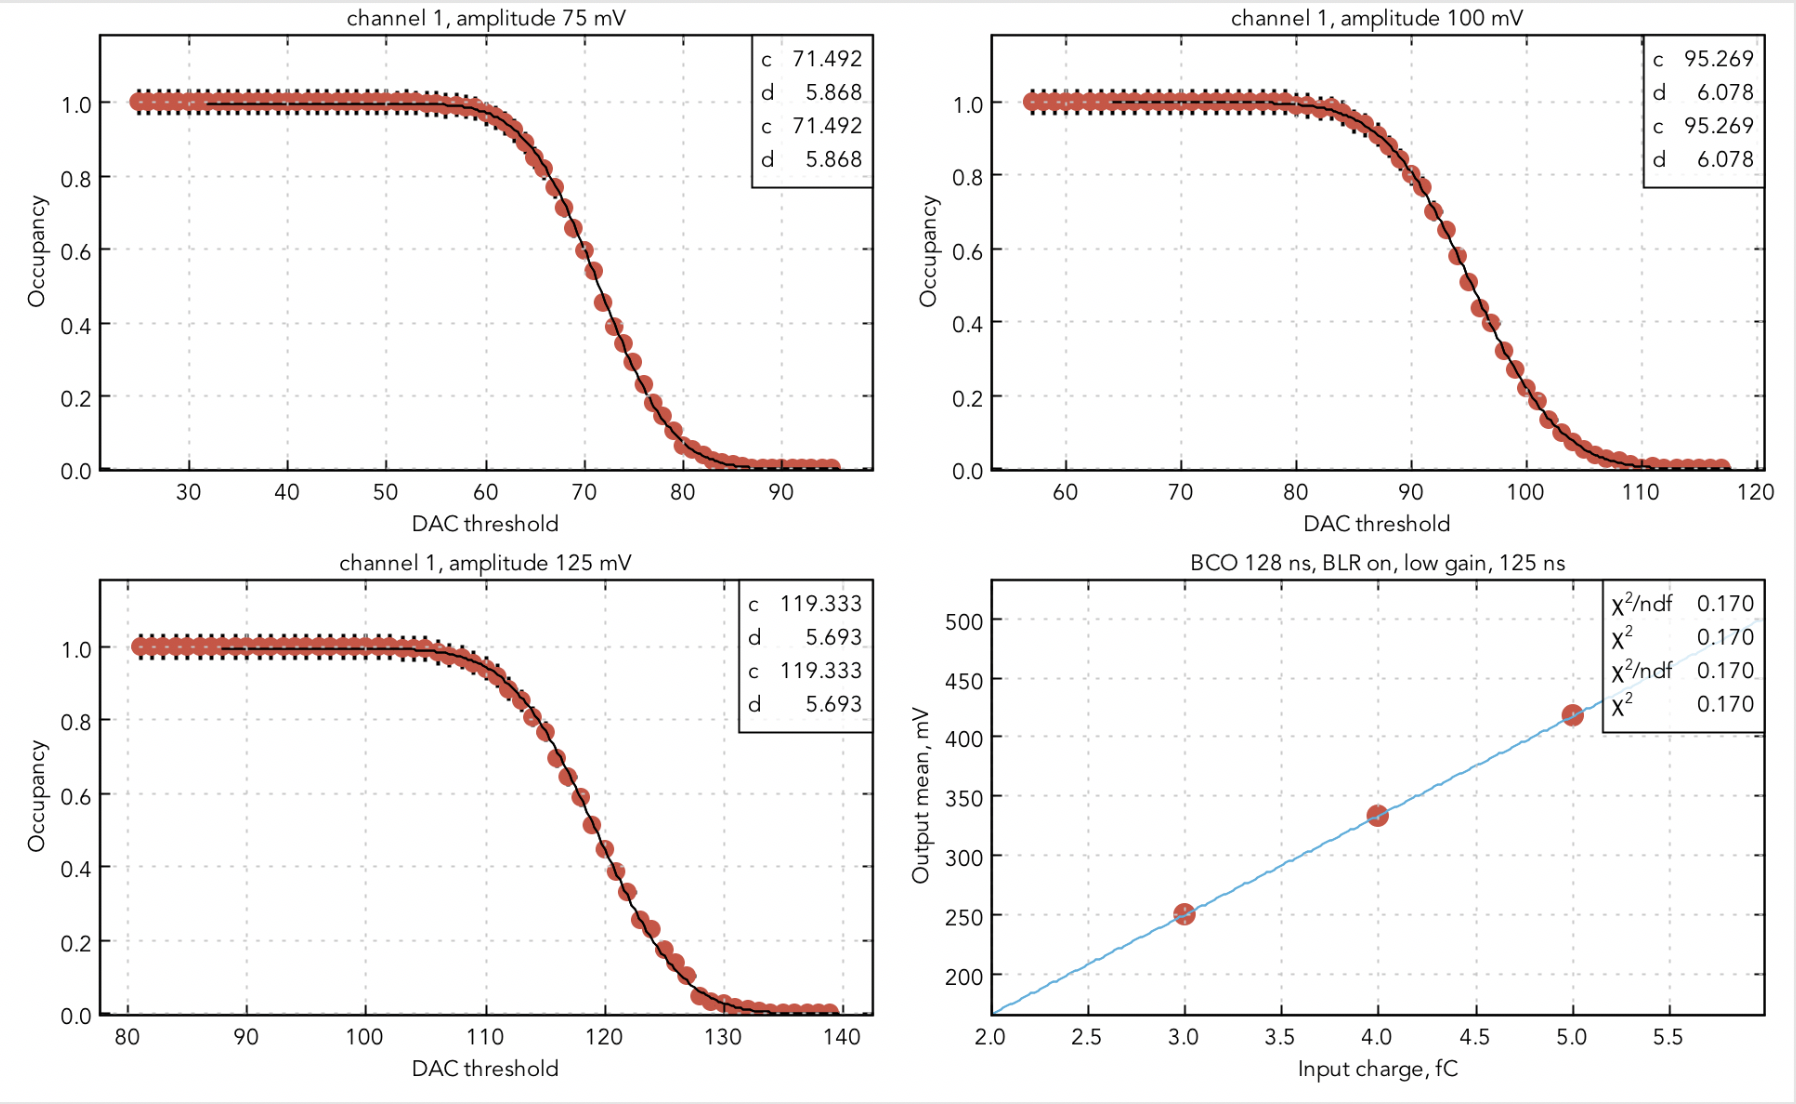
\includegraphics[width=1.0\columnwidth,keepaspectratio]{threshold-scan.png}
	\caption{Threshold scan on a single representative SVT channel.}
	\label{fig:threshold-scan}
\end{figure}

The output signals from the FSSR2 chip can be converted to charge using either internal or external calibration pulses. Because external pulser can be set to higher frequency than internal pulser without affecting the calibration process, external pulser circuit was added to the HBCB and the VSCM. Noise is measured using external, low frequency calibration charge injected in the absence of signal. The injected charge is shaped and amplified in the analog circuitry to form an output signal. The discriminator threshold determines whether or not the output signal corresponded to a hit. The probability that the injected charge produces a hit depends on the setting of the discriminator threshold. The average hit probability is measured by repeating the process of injecting charges and counting the fraction of readout triggers that produced a hit. This measurement is repeated over a range of threshold settings to produce an occupancy plot. 

The occupancy plots are measured setting the pulser amplitude at fixed values and changing the comparator thresholds. Each point of an occupancy plot represents the percentage of times that the comparator fires for a certain value of injected charge. In Fig.~\ref{fig:threshold-scan} presented three occupancy plots taken at different pulser amplitudes and the response plot showing the linear dependence of the output pulse height on the input charge in the operation region of the preamplifier. In between the high and low threshold regions, the occupancy curve is described by an error function, or S-curve, which can be fitted to the occupancy histogram for each channel, producing a mean value (discriminator threshold) and standard deviation (noise). The conversion from mV to electrons is performed considering a nominal value for the FSSR2 injection capacitance of 40~fF. 

\begin{figure}[hbt] 
	\centering 
	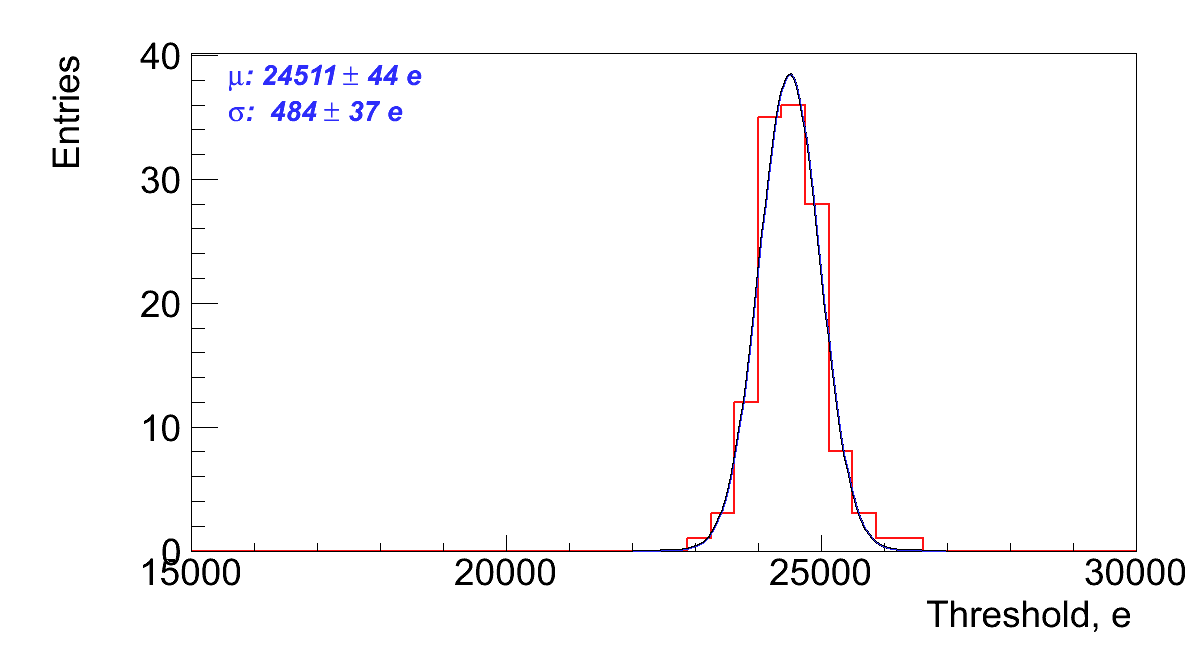
\includegraphics[width=0.8\columnwidth,keepaspectratio]{thrdisp.png}
	\caption{Typical threshold dispersion within a chip.}
	\label{fig:thrdisp}
\end{figure}

Threshold dispersion is defined to be a standard deviation of the distribution of means obtained from the parameters of the complementary error function fit. The noise and threshold dispersion constants for each individual detector channel are measured and the values are used by the zero-suppression algorithms implemented in the core logic of the FSSR2 and by calibration procedures to identify defective channels. A comparison of the noise for 33~cm strips with the threshold spread demonstrates that the threshold spread is negligible compared to the noise and does not affect the efficiency and noise occupancy (see Fig.~\ref{fig:thrdisp}). The threshold dispersion agrees with expectations for the FSSR2 chip for the chosen settings.

SVT calibration data are stored in CLAS12 calibration database. The channel calibration table has columns corresponding to sector, layer, chip ID, mean, channel status (good, noisy, open, dead, or masked), equivalent noise charge (ENC), gain, offset, Vt50 (threshold at 50$\%$ occupancy), and the threshold. There are 21504 rows in the channel calibration table. The ENC and gain are calculated using a calibration amplitude equal to 100 DAC.
The chip calibration table has columns corresponding to layer, sector, chip ID, ENC (electrons), gain (mV/fC), offset (mV), the threshold at 50$\%$ occupancy (Vt50, mV), threshold dispersion (electrons), chip gain (low, high), BLR mode (off, on), BCO time (ns), shaper time (ns), 8 ADC thresholds in DAC. There are 168 rows in the chip calibration table. 

